\documentclass[a4paper,10pt, oneside]{book}

\usepackage{polyglossia}  % multilingual support
\usepackage{xcolor}  % can't use color with polyglossia

\usepackage{bidipoem}

\usepackage{tabularx}  % Needs to be above longtable
\usepackage{longtable}  % Tables that split over a pagebreak.
\usepackage{booktabs}  % Modern-style tables.
\usepackage{multirow}  % Merge cells in a table: provides \multirow, \multicolumn
\usepackage{array}  % Allows justification to be specified in tabularx columns.

\usepackage{arydshln}  % For dashed lines.

\usepackage[obeyspaces]{url}  % Use urls in text and captions with sensible linewrap.
\urlstyle{rm}  % Set urls in roman.

\usepackage{graphicx}  % Allows images to be inserted.
\usepackage{appendix}  % Provides additional appendixing capabilities.
\usepackage[labelfont=bf,textfont=it]{caption} % Set properties for captions - wider margins, smaller font, bold figure label, etc.

\usepackage{natbib}

\usepackage{cleveref}


\interfootnotelinepenalty=10000 % prevents the footnote from breaking across pages
% http://tex.stackexchange.com/questions/32208/footnote-runs-onto-second-page

% Thanks to Manas Tungare (http://manas.tungare.name/software/latex) for these settings.
\setlength{\paperwidth}{210mm}
\setlength{\paperheight}{297mm}

\setlength{\textwidth}{160mm}
\setlength{\textheight}{247mm}

\setlength{\evensidemargin}{1in}
\setlength{\oddsidemargin}{0in}
\setlength{\topmargin}{-0.5in}

%--------------------------------
%%% Font definitions %%%
%--------------------------------
% Note that these definitions malfunction if used in \chapter.
\defaultfontfeatures{Mapping=tex-text}
\setmainfont{Charis SIL}  % Set the default font for the document. = \setdefaultfont
% Footnotes will by default also use this font -- http://tex.stackexchange.com/questions/4779/how-to-change-font-family-in-footnote).
\defaultfontfeatures{Scale=MatchLowercase}  % needs to be below main font declaration

\setsansfont{Liberation Sans}
\setmonofont{Liberation Mono}

\setmainlanguage{english}
\setotherlanguage{arabic}

\newfontfamily\arabicfont[Script=Arabic, Scale=2]{Scheherazade} % Arabic transcription -- coloured black, double size.
% One font needs to be called \arabicfont in order for XeTeX to load Arabic-related hyphenation and other stuff.
%  The default \textarabic will use this \arabicfont.  Use the \begin{Arabic} ..... \end{Arabic} environment for longer stretches (eg paras).
% Use \textarabic{\aemph{با}} to give overline emphasis.
% Omitting Script=Arabic for Amiri or Granada will mean that letters are written in their standalone forms, not connected.  (Omitting Script=Arabic for Scheherazade seems to cause no problem, though.)

\newfontfamily\citationfont[Script=Arabic, Scale=1.5]{Scheherazade}  % Citations, or stand-alone Arabic script in the middle of Roman script -- coloured black, one-and-a-half size.
\newcommand\AS[1]{{\citationfont\RLE{#1}}}
% \RLE (from the bidi package, which polyglossia loads automatically) is to allow multiple words of Arabic to be written right-to-left -- if omitted, each word in the sequence will be written RTL, but the sequence as a whole will be written LTR.

%You can either, as above, define a new \fontfamily, and then use it in a \newcommand, or you can, as below, include the font in the \newcommand by calling \fontspec directly.

\newcommand\Atitle[1]{{\fontspec[Script=Arabic, Scale=2]{GranadaKD}\RLE{#1}}}  % Arabic transcription for titles - uses a version of Granada which has been extended to include glyphs for Swahili.

\newcommand\Am[1]{{\fontspec[Script=Arabic]{Amiri}\RLE{#1}}} % Examples using Amiri --  if using Scheherazade's default scale, set Scale=0.8 here.

\newcommand\Tr[1]{{\fontspec[Scale=0.9, Color=666666]{Linux Biolinum O}#1}}   %  Transliteration -- Biolinum handles diacritics well.  Coloured black, slightly less than normal size.
% Scale=1 is required because of Scale=MatchLowercase - otherwise the size is too large.

\newcommand\I[1]{{\fontspec[Scale=1, Color=blue]{Linux Biolinum O}#1}}  % Epenthetic letters in the transliteration -- coloured blue, normal size.

\renewcommand\S[1]{{\fontspec[Color=00BB33, Scale=1]{Linux Biolinum O}#1}}  % Standard spelling -- coloured green, normal size.
% Command \S is used for something else, hence \renewcommand.  Bad idea -- needs to be changed to \Sspell or something.

\newcommand\E[1]{{\fontspec[Scale=0.9, Color=666666]{Liberation Serif Italic}#1}}  % English translation layer -- coloured grey, slightly less than normal size.

\newcommand\FN[1]{{\fontspec[Color=00BB33]{Liberation Serif Italic}#1}} % Standout type in footnotes -- coloured green, normal size.

\newcommand\EBG[1]{{\fontspec{EB Garamond 12 Italic}#1}}  % Garamond test.

% Older versions:
% \newfontfamily{\Tr}[Scale=0.9, Color=00BB33]{Linux Biolinum O}
% This can be used as \Tr{text}.  But this will change the font outside the argument until the end of that stretch.
% This doesn't show up in the poemlines, because they are self-contained, but it does show up in connected text.
% To avoid this, and have the font only changed within the argument, use \newcommand as above.

%----------------------------------------
%%% End of font definitions %%%
%----------------------------------------

% titlesec commands have to come after 
% \setmainlanguage{english}
% \setotherlanguage{arabic}
% above, otherwise they are overridden and have no effect.
\usepackage{titlesec}  % Allow the chapter/section heading settings to be fine-tuned.
\titleformat{\chapter}[display]{\normalfont\large}{\bfseries\chaptertitlename\ \thechapter}{10pt}{\LARGE\itshape}[\vspace{2ex}\titlerule]  % 10pt is the space between chapter and chapter name.  [display] sets the chapter and chapter name on separate lines.  The square brackets at the end draw a line under each chapter name, with 2ex gap from the name.
\titlespacing{\chapter}{0pt}{0pt}{10pt}  % First is indent from the side, second is length down from the top, third is gap between heading and text.
\titleformat{\section}[block]{\normalfont\large\itshape}{\itshape\thesection}{1em}{}  % 1em is the space between section number and section name.  [block] sets the section and section name on the same line.

\renewcommand\thefootnote{\textcolor{red}{\arabic{footnote}}}  % Alter the colour of the footnote markers - thanks to Gonzalo Medina (http://tex.stackexchange.com/questions/26693/change-the-color-of-footnote-marker-in-latex#26696).

%Redefine the underscore command
\let\underscore\_
\newcommand{\myunderscore}{\renewcommand{\_}{\underscore\hspace{0pt}}}
%Issue the changed underscore command to the whole document.
\myunderscore
% Or:
% \usepackage{underscore}  % Escape _ so that it doesn't cause compile errors.

\setlength{\parindent}{0in}  % no paragraph indents
\setlength{\parskip}{2ex}  % put a linespace between paragraphs

\title{\textbf{Writing and transliterating\\Swahili in Arabic script\\with \textit{Andika!}}}
\author{Kevin Donnelly\thanks{kevin@dotmon.com}}
\date{}



\begin{document}
\frenchspacing


% make the title page
\begin{titlepage}
\begin{center}

{\Huge\textbf{Writing and transliterating\\Swahili in Arabic script\\with \textit{Andika!}}} \\
[3cm]

{\LARGE{Kevin Donnelly}} \\
[3cm]

{\Large{2014}} \\
[10cm]

This manual is a work-in-progress.\\
The most important part at the moment is Appendix A, giving installation instructions.\\
\end{center}
\end{titlepage}


\chapter{Introduction}
\label{s:intro}

For centuries, Swahili was written in Arabic script, and hundreds of manuscripts in collections around the world testify to its long tradition of written literature. Over the last century, however, Swahili in Roman script has become the norm.

\textbf{Andika!} (meaning \textbf{Write!} in Swahili) is a set of tools to make Swahili in Arabic script as easy to use as Swahili in Roman script - it is equally easy to read and write the the language in either script. The tools, based on the work of Marehemu Mu'allim Sheikh Yahya Ali Omar \citep{Omar1997} provide a consistent, standardised transliteration of Swahili in Arabic script, and a one-to-one mapping of this to Swahili in Roman script.

All the tools are available under version 3 of the Free Software Foundation's General Public License,\footnote{http://www.gnu.org/licenses/gpl.html} which means they can be adapted and extended as required by the user, subject to the same license being used for any new version thus created.


\chapter{Benefits}
\label{s:benefits}

\begin{itemize}
 \item Swahili manuscripts in Arabic script can be directly transcribed and made available in digital format. At present, most Swahili literature from earlier periods has only been published in Roman transliteration. The third image in the slideshow above shows part of a manuscript rendering of Bajuni fishing songs, transcribed letter-for-letter from the manuscript.

 \item A direct transcription can be augmented with a fully-vocalised Arabic transcription, a close phonetic transliteration, a transliteration in the standard Roman orthography, and so on, according to taste. The tools allow much of these to be generated automatically, reducing the effort this would otherwise involve.

 \item Apart from allowing easier typesetting and dissemination, having manuscripts in digital form will make it possible for the first time to use computers to look at word frequency, stylistic variation, etc, within the texts, to build corpora for classical Swahili, and so on.

 \item New writing in Swahili can be composed in Arabic script and published easily via word-processors, webpages, or pdfs created by typesetting systems such as LaTeX.

 \item The ability to convert Arabic script at any time into Roman script means that there is very little overhead involved in choosing to write Swahili in Arabic script. Material can be produced simultaneously in both scripts with the minimum of effort (although the converted text will need minor editing to cover such things as capital letters, which do not exist in Arabic script).

 \item Existing Swahili content in Roman script can be converted to Arabic script, making it possible to reuse content already published in Roman script. This means that large amounts of material in Arabic script can be be made available very quickly - it is not necessary to create them specially.

 \item The conversion tools include cut-and-paste boxes for small amounts of text, a Roman-to-Arabic converter for entire webpages, and offline converters for bulk conversion of text.

 \item The Arabic-to-Roman conversion can be extended to provide a variety of different transliterations (eg kh or x for \AS{خ} instead of the standard h).

 \item The Roman-to-Arabic conversion can be adjusted to convert numerals, to add or remove markers such as \textit{sakani} (\textit{sukun}), and so on.
\end{itemize}


\chapter{Getting started}

Detailed instructions for installing \textbf{Andika!} and the other software it requires are in Appendix A..

It's very easy to get started. The most important thing is to install a font that will show all the Arabic characters used in Swahili - once that is done, you can use all the resources on this website.

The best font option at the minute is Scheherazade - to get the most recent version, download ScheherazadeRegOT-1.005.zip from this page, and unzip it. Then double-click the file ScheherazadeRegOT.ttf to install the font on your computer.

You can type Swahili in Arabic script directly into a Linux computer using a standard UK keyboard. Input speed is comparable to typing in Roman script. The Swahili keyboard section includes simple step-by-step instructions for enabling a Swahili keyboard layout on Ubuntu running KDE, and for making changes to it if you have a non-UK keyboard.

Alternatively, if you don't want to do that just yet, go to the Roman to Arabic section. There, you can type into a box in Roman script and have the input converted into Arabic script, or you can input a web address and have that whole page converted into Arabic script. The offline converters allow multiple files to be converted easily.

You can cut and paste the converted Arabic text into a word-processor. See the LibreOffice tab in the Swahili keyboard section.

You can also go to the Arabic to Roman section to convert Arabic script into Roman script (standard Swahili orthography by default, but options are available to add various diacritics to the transliteration). The offline converters allow a transcription of an existing Swahili manuscript in Arabic script to be automatically transliterated into Roman script.

The Spelling conventions section gives suggestions for using Arabic script with current-day Swahili, with many examples of how the Arabic script maps to the Roman script.

The section on Typesetting poetry shows how Swahili poetry manuscripts in Arabic script can be transcribed digitally to produce attractive output in various formats, with the added benefit that the contents of the manuscripts are then available for computer analysis of language, vocabulary, word-frequency, etc. 

% \begin{longtable}{rrl} 

% \makebox[8cm][r]{} & & \makebox[8cm][r]{} \\ 

% \textarabic{تَانْيَامَا حَتَ لِنِ} & \textarabic{كُنْيَمَا نِ مٖػوْكَ} & \textarabic{١} \\* 
% \Tr{ṯānyāmā ḥaṯa lini} & \Tr{kunyamā ni mekʲūka} & \\* 
% \multicolumn{2}{r}{\S{kunyamaa nimechoka * t'anyamaa hata lini}} & \S{1a/b} \\* 
% \multicolumn{2}{r}{\E{I am weary of staying silent. For how much longer am I to remain dumb?}} & \\[2mm] 
% \textarabic{كُوَأٗنَ نَ تَمَانِ} & \textarabic{وَنَنْڠُ هُنِئٖپُوْكَ} &  \\* 
% \Tr{kuwaona na ṯamāni} & \Tr{wanangu huniepūka} & \\* 
% \multicolumn{2}{r}{\S{wanangu huniepuka * kuwaona natamani}} & \S{1c/d} \\* 
% \multicolumn{2}{r}{\E{My own children avoid me, though I long to see them.}} & \\[2mm] 
% \textarabic{سِوَنْڠُ نِ وَ وٖنْدَانِ} & \textarabic{والُوْبَاكِ كُنِشِكَ} &  \\* 
% \Tr{siwangu ni wa wenḏāni} & \Tr{wālūbāki kunishika} & \\* 
% \multicolumn{2}{r}{\S{walobaki kunishika * si wangu ni wa wendani}} & \S{1e/f} \\* 
% \multicolumn{2}{r}{\E{And those who remain to embrace me are not my own, but are the offspring of others.}} & \\[2mm] 
% \textarabic{مْبُوْنَ هُنِپِجَ زِتَ} & \textarabic{مِمِ نِ مٖوَتٖنْدَانِ} &  \\* 
% \Tr{mbūna hunipija ziṯa} & \Tr{mimi ni mewaṯenḏāni} & \\* 
% \multicolumn{2}{r}{\S{mimi nimewatendani * mbona hunipija zita}} & \S{1g/h} \\* 
% \multicolumn{2}{r}{\E{What have I done to you? Why do you wage war on me?}} & \\[2mm] 
% \\[8mm] 
% 
% \textarabic{وَانَ وَ أُسْوَاحِلِنِ} & \textarabic{وَنَانْڠُ مِمِ وَ دَمُ} & \textarabic{٢} \\* 
% \Tr{wāna wa uswāḥilini} & \Tr{wanāngu mimi wa ḏamu} & \\* 
% \multicolumn{2}{r}{\S{wanangu mimi wa damu * wana wa Uswahilini}} & \S{2a/b} \\* 
% \multicolumn{2}{r}{\E{My own flesh and blood, the children of Swahililand,}} & \\[2mm] 
% \textarabic{يَا كُنِيُوَ نِ نَانِ} & \textarabic{أَصِلِ هَوَنَ هَامُ} &  \\* 
% \Tr{yā kuniyuwa ni nāni} & \Tr{aṣili hawana hāmu} & \\* 
% \multicolumn{2}{r}{\S{asili hawana hamu * ya kuniyuwa ni nani}} & \S{2c/d} \\* 
% \multicolumn{2}{r}{\E{are uninterested in knowing who I am,}} & \\[2mm] 
% \textarabic{نَ وَنَ وَ مَجِرَنِ} & \textarabic{وَمٖنَتِيَ قَؤُمُ} &  \\* 
% \Tr{na wana wa majirani} & \Tr{wamenaṯiya qaumu} & \\* 
% \multicolumn{2}{r}{\S{wamenatiya kaumu * na wana wa majirani}} & \S{2e/f} \\* 
% \multicolumn{2}{r}{\E{and have left me to other peoples, and to the children of neighbours.}} & \\[2mm] 
% \textarabic{مْبُوْنَ هُنِپِجَ زِتَ} & \textarabic{كُوْسَ لَنْڠُ كُوْسَ ڠَانِ} &  \\* 
% \Tr{mbūna hunipija ziṯa} & \Tr{kūsa langu kūsa gāni} & \\* 
% \multicolumn{2}{r}{\S{kosa langu kosa gani * mbona hunipija zita}} & \S{2g/h} \\* 
% \multicolumn{2}{r}{\E{What kind of fault is my fault? [O my children] why do you continue waging war on me?}} & \\[2mm] 
% \\[8mm] 
% 
% \textarabic{وَلَ سِنَ پُنْڠُوَنِ} & \textarabic{مِمِ مَامٖنُ سِتَاسَ} & \textarabic{٣} \\* 
% \Tr{wala sina punguwani} & \Tr{mimi māmenu siṯāsa} & \\* 
% \multicolumn{2}{r}{\S{mimi mamenu sit'asa * wala sina punguwani}} & \S{3a/b} \\* 
% \multicolumn{2}{r}{\E{I am your mother and am not yet infertile, nor has my ability to reproduce diminished.}} & \\[2mm] 
% \textarabic{نَ كُنْڠِنٖ زِسِوَنِ} & \textarabic{نِ مٖزَا وَ مَمْبَاسَ} &  \\* 
% \Tr{na kungine zisiwani} & \Tr{ni mezā wa mambāsa} & \\* 
% \multicolumn{2}{r}{\S{nimezaa wa Mambasa * na kungine zisiwani}} & \S{3c/d} \\* 
% \multicolumn{2}{r}{\E{I have given birth to children in Mambasa, and in the other islands [of the Swahili],}} & \\[2mm] 
% \textarabic{نَ زِيُوْنْڠُوْزِ وَدِنِ} & \textarabic{نِزٖ وَنَ سِيَاسَ} &  \\* 
% \Tr{na ziyūngūzi waḏini} & \Tr{nize wana siyāsa} & \\* 
% \multicolumn{2}{r}{\S{nizee wanasiyasa * na ziongozi wa dini}} & \S{3e/f} \\* 
% \multicolumn{2}{r}{\E{to politicians and to religious leaders,}} & \\[2mm] 
% \textarabic{نَ مَاشُجَا وَ زِتَ} & \textarabic{مَافُنْدِ وَ كُلَ فَنِ} &  \\* 
% \Tr{na māshujā wa ziṯa} & \Tr{māfunḏi wa kula fani} & \\* 
% \multicolumn{2}{r}{\S{mafundi wa kila fani * na mashujaa wa zita}} & \S{3g/h} \\* 
% \multicolumn{2}{r}{\E{to craftsmen in every field, and to war heroes.}} & \\[2mm] 
% \\[8mm] 
% 
% \textarabic{پِيَ مْوٖنْڠٗ عَثْمَانِ} & \textarabic{نْدِمِ مَامَاكٖ مُيَاكَ} & \textarabic{٤} \\* 
% \Tr{piya mwengo 'ath}\I{u}\Tr{māni} & \Tr{nḏimi māmāke muyāka} & \\* 
% \multicolumn{2}{r}{\S{ndimi mamake Muyaka\footnote{Bwana Muyaka was the outstanding Swahili poet of 19th century Mombasa.  After his death many of his verses were recalled by Mu'allim Sikujua Abdallah al-Batawi (died 1890) and transcribed with annotations by W.E. Taylor (1856-1927). After Taylor’s death his papers were acquired by the library of the School of Oriental and African Studies (SOAS), London.} * pia Mwengo Athumani\footnote{Mwengo Athmani: this 18th century poet from Pate composed the {\FN{Utendi wa Tambuka}} (\textit{The Epic of Heraklios}).}}} & \S{4a/b} \\* 
% \multicolumn{2}{r}{\E{I am the mother of Bwana Muyaka, and of Mwengo Athmani also,}} & \\[2mm] 
% \textarabic{نَ وٖنْڠِ وَاكٖ وٖنْدَانِ} & \textarabic{نَ زَهِدِ كَذَلِكَ} &  \\* 
% \Tr{na wengi wāke wenḏāni} & \Tr{na zahiḏi kadhalika} & \\* 
% \multicolumn{2}{r}{\S{na Zahidi\footnote{Zahidi: see El-Maawy (2008).} kadhalika * na wengi wake wendani}} & \S{4c/d} \\* 
% \multicolumn{2}{r}{\E{and of Zahidi too, and many of his contemporaries,}} & \\[2mm] 
% \textarabic{وٗتٖ مْبوَا مُوْيَ قَرِنِ} & \textarabic{عالى كُوْتِ نَ مَتَاكَ} &  \\* 
% \Tr{woṯe mbwā mūya qarini} & \Tr{'ālı̄ kūṯi na maṯāka} & \\* 
% \multicolumn{2}{r}{\S{Ali Koti\footnote{Ali Koti of Pate: see Chiraghdin (1987: 31-7).} na Mataka\footnote{Bwana Mataka’s full name is Muhammad bin Shee Mataka al-Famau (1825-1868). He was ruler of Siyu, as was his father. His mother was Mwana Kupona, famous for the poem of advice written to her daughter. Bwana Mataka died in Mombasa’s fort while imprisoned by the Busa‘idi.
% } * wote mbwa moya karini}} & \S{4e/f} \\* 
% \multicolumn{2}{r}{\E{Ali Koti and Mataka, all from just one century,}} & \\[2mm] 
% \textarabic{وَ كَوَا كَمَ نْيوتَ} & \textarabic{وَلِتُوْكَ مَاتُوْمبونِ} &  \\* 
% \Tr{wa kawā kama nı̄ūṯa} & \Tr{waliṯūka māṯūmbūni} & \\* 
% \multicolumn{2}{r}{\S{walitoka matumboni * wakawaa kama nyota}} & \S{4g/h} \\* 
% \multicolumn{2}{r}{\E{they emerged from my womb, and shone like stars.}} & \\[2mm] 
% 
% \end{longtable}

\chapter{Slideshow images}

The images in the slideshow give examples of various pieces of Swahili written in Arabic script. The intention is to show that the Andika! tools can cope with a variety of different requirements - all the copies are transcribed letter-for-letter from the originals.

Image 1
The word andika! (write!) is shown in various Arabic fonts, giving some idea of the variety and expressiveness of the script. Virtually all of these fonts, however, have been designed for Arabic only, and need characters added to them before they are useable with Swahili. See the Fonts tab in the Keyboard section.

Image 2
A copy of the specimen text from Appendix C of \citet{Omar1997}, which they included to show how their system would look in practice. The text is a section from \citet{Omar1998}.

Image 3
A section of the Swahili Wikipedia page on \AS{أُتَمَدُونِ} (\textbf{utamaduni}, \textit{culture}), converted using \textbf{Andika!} conventions - see the section Spelling conventions.

Image 4
A copy of the first few verses from a manuscript written by Sheikh Yahya himself, giving a transcription of Bajuni fishing songs -- see \citet{Donnelly1982}.  The Arabic script in this manuscript differs in a number of minor respects from the one in \citet{Omar1997}.  The Roman conversion in this case uses various diacritics to reconcile the manuscript's representation of the Bajuni dialect with standard orthography. This close transcription (like the default standard transcription) is generated automatically, and can be made the default. Further converters can be set up to reflect other transcription conventions.

Image 5
A copy of verses 3-5 of \citet{Harries1967}.  This is one of the few books of Swahili classical poetry to include the text in Arabic script alongside the Roman transcription, in this case a photocopy of a copy of the original manuscript made by Sheikh Yahya. The Arabic script in this manuscript is less well-adapted to Swahili - for instance, \textit{o} is not used consistently. The Roman transcription is Harries' own - a generated close transcription might be:

% http://texblog.org/2013/02/27/on-paragraphs-in-texlatex/
\hangindent=3cm  % controls the amount of indentation from left (positive value) or right (negative value).
\hangafter=0  % controls the number of full-width lines before/after changing the indent (\hangindent) - a positive number produces full-width lines at the beginning, whereas a negative number produces them at the end. 0 means we want them all indented, including the first line.
\Tr{
dōla mbili ziliwāna * shikuwe nā simba mbawāna\\
kamaṯezo kushindāna * mṯāna nalayliyā\\
zikiṯimu siku ṯāṯu * shikuwe kaṯaka wāṯu\\
kuṯukuwa chāke kiṯu * nḡūbe kay nunuliyā\\
kaṯiya ngūbe ndiyāni * mema āsiyu lahāni\\
simba shı̄ kabaı̄ni * mpāni ngūbe mmuyā
}\normalfont


\chapter{Typing Swahili in Arabic script}

The main aim of Andika! is to enable Swahili manuscripts in Arabic script to be transcribed digitally in Arabic script - see the section Typesetting poetry. (A second aim, enabling Arabic script to be used easily for current-day writing of Swahili, is covered in the section Spelling conventions. Round-trip conversion between Arabic and Roman scripts is a useful by-product of these two aims, and is covered in the Arabic to Roman and Roman to Arabic sections.)

The keyboard layout proposed here should enable most historical manuscripts to be transliterated letter-for-letter, and since it uses a standard keyboard, and links the Arabic letters to their Roman equivalents, it is easy to start using immediately.
Initial requirements

It is assumed that you have a computer running Ubuntu, and are broadly familiar with how to use it. Ubuntu is a GNU/Linux distribution launched by a South African, Mark Shuttleworth, and the name is cognate with Swahili \AS{أُوتُ} (\textbf{utu}, \textit{humanity}).

If you are not currently using Ubuntu, it is possible to run it in a virtual machine on top of Microsoft Windows or Apple Mac OS.

It is assumed that you are using the KDE desktop environment, and the instructions here apply to that. Similar options, however, are available if you are using other desktops such as GNOME or Unity. If you wish to use KDE as your own desktop environment, just install the kubuntu-desktop package in Ubuntu.

It is assumed that you are familiar with the basic conventions of the Arabic alphabet (eg the different letter-shapes).
Install a font

In order to see the Arabic script properly, your computer must be able to access a font that includes Arabic letterforms (glyphs). Many fonts nowadays will include some Arabic glyphs, but their attractiveness and coverage varies widely - for instance, many fonts do not include \AS{پ} (p) or \AS{ڠ} (g). If you are seeing squares or boxes in the Arabic script, the reason is that the font you are using is missing glyphs.

The best font option currently is Scheherazade, created by Bob Hallissy and Jonathan Kew. To get the most recent version, download ScheherazadeRegOT-1.005.zip from this page, and unzip it. Then double-click the file ScheherazadeRegOT.ttf to install the font on your computer. In Ubuntu, it will be installed into \textit{/usr/local/share/fonts/}.


\chapter{Using the keyboard}

The keyboard (Figure \ref{fig:kblayout})\footnote{I am grateful to Wikimedia for the original layout image.} uses the following layout  to make Arabic glyphs available in Swahili.

\begin{figure}[h]
 \centering
 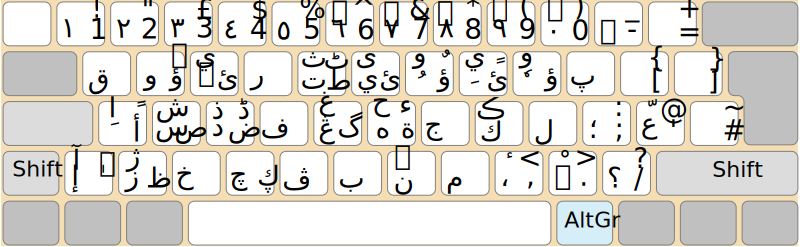
\includegraphics[keepaspectratio=true, scale=0.7]{./images/Swahili_keyboard.png}
 % Swahili_keyboard.png: 797x246 pixel, 90dpi, 22.50x6.94 cm, bb=0 0 638 197
 \caption{Keyboard layout for writing Swahili in Arabic script}
 \label{fig:kblayout}
\end{figure}

As can be seen from Figure \ref{fig:kblayout}, up to four glyphs may be accessed from one key.  To access the contents of each key, the \textbf{Shift} and \textbf{AltGr} keys are used in combination where appropriate, as shown below:

\begin{figure}[h]
 \centering
 \includegraphics[keepaspectratio=true, scale=0.8]{./images/key.png}
 % key.png: 562x100 pixel, 90dpi, 15.86x2.82 cm, bb=0 0 450 80
 \caption{Accessing the contents of keys}
 \label{fig:key}
\end{figure}


Layout conventions

The basic idea behind the keyboard layout is that the relevant Arabic letter will usually be produced by pressing the same key that produces the Roman letter. Additional points:

Digraphs such as \textbf{dh gh th} are placed on the same key as \textbf{d g t}, and accessed using the \textbf{Shift} key.

The digraph \textbf{ch} is accessed using the \textbf{C} key.

The digraph \textbf{sh} is accessed using the \textbf{Shift+S} keys.

The occasionally-used digraph \textbf{kh} is accessed using the \textbf{X} key.

Arabic letter variants are placed on the same key where possible, eg \AS{ي} and \AS{ى}.

Similar sets of Arabic letters are placed consistently - for instance, the pharyngeal consonants \AS{ص ض ط ظ} are all accessed using the \textbf{AltGr} key, as are \AS{ؤ ئ}, and the alveolar consonants \AS{ٹ ڈ} used in Mombasa Swahili are accessed using the \textbf{Shift+AltGr} keys.

Long and short vowels are located on the same key, with the long vowel accessed by \textbf{Shift}, and the vowel-carrier accessed by \textbf{AltGr}, so for instance the \textbf{U} key produces \AS{ُ } and \textbf{Shift+U} produces \AS{و}, with \textbf{AltGr+U} producing \AS{ؤ}.

The letters \AS{و ي} are also available on \textbf{y w} for use when they represent semi-vowels.

Non-alphabetic characters from the UK keyboard are available via \textbf{AltGr} and \textbf{AltGr+Shift}.


Changing the layout

(Note that this layout can be easily changed if it does not suit your needs - a section on how to do this will be added later.)
Perhaps put this in an Appendix -- see Appendix \ref{app:2}.

Configure LibreOffice

In order to test the keyboard, we will configure LibreOffice to display text in Arabic script. Launch LibreOffice, and click on Tools → Options → Language Settings → Languages:
Set CTL to Arabic (Oman) and tick Enabled for complex text layout (CTL). This will create two new buttons on the icon bar, one for left-to-right typing, and one for right-to-left typing:
Click the RTL button to move the cursor over to the right-hand side of the line.

There appears to be a bug in LibreOffice whereby the first letters you type in RTL mode do not use the font you have selected, but the system font (in my case, Deja Vu Sans), so the easiest thing to do is to type something first and then change the font. Switch to the Swahili keyboard (Ctrl+Alt+k), type m, i, Shift+i, m, i, and press Return. Then press Ctrl+a, choose Scheherazade as the font, and set the font size to something large, like 26. You should now have something like this:
showing the Swahili word mimi (I, me) in Arabic script.

Continue typing the following words, ignoring commas, and pressing Return after each one:
s, a, Shift+a, s, a - sasa (now)
k, Shift+. (period), w, e, Shift+e, l, i - kweli (truly)
l, u, Shift+u, Shift+g, a - lugha (language)
n, Shift+n, o, Shift+o, m, b, e - ng'ombe (cattle)
AltGr+a, u, m, e, f, i, Shift+i, k, a - umefika (you have arrived)

You should now have something like this:
Other LibreOffice settings

On this site, the Arabic font has purposely been made quite large, so that the details of the text can be seen. You may wish to make the font size smaller. In Arabic, where vowel signs are only rarely used, reading the text is possible at quite small font sizes. In Swahili, however, the vowel signs are essential, so the same reductions in font size are not possible (I find 15pt to be the level at which legibility begins to be impaired, but your eyes might be better than mine!). In typesetting poetry, of course, the lines are short, and accuracy is improved by having a large font.

Some of the vowel signs (eg \AS{ٖ} under a word-final \AS{ي}) can get hidden below the visible window of the line, so it is often useful to set the line-spacing of the LibreOffice document to 1.5: Ctrl+a, then click on Format → Paragraph, select 1.5 linee under Line spacing, and then click OK.

Number-handling when using the Swahili keyboard will depend on the settings under Tools → Options → Language Settings → Complex Text Layout . If you wish to use both Arabic-Indic numerals (on the numeral keys) and Western-Arabic numerals (AltGr+numeral), ensure Arabic or System is chosen here. The other two settings will convert Western-Arabic numerals to their Arabic-Indic equivalents.


\chapter{Fonts}
\label{mans:fonts}

There are a couple of dozen Arabic fonts available in the packages fonts-kacst and fonts-arabeyes, but virtually all of these fonts have been designed for Arabic only, and need characters added to them before they are useable with Swahili.

The only fonts that will work properly with Swahili at the time of writing are Scheherazade (Bob Hallissy and Jonathan Kew), Amiri (Khaled Hosny), and the fonts from the PakType project (of which perhaps Tehreer is the most attractive). All of these are in the Naskh style.

The main stylistic differences between Scheherazade and Amiri are that Amiri contains all the Arabic presentation forms (character combinations), making for more attractive text. For instance, Amiri \Am{وَلِتُمئَِ} (\textit{walitumia}, they used), compared to Scheherazade \AS{وَلِتُمئَِ}, has the letters \textit{ltm} combined in one ligature.

However, Amiri places all the vowels at the same height from the main letter, eg \Am{كُبٗرٖيشَ} (\textit{kuboresha}, to boost) compared to Scheherazade \AS{كُبٗرٖيشَ}, and \Am{وَنَسَيَانْسِ} (\textit{wanasayansi}, scientists) compared to Scheherazade \AS{وَنَسيَانْسِ}. This can lead to the upper vowels from the current line of text colliding with the lower vowels from the previous line, so Amiri may be more appropriate for use with text that is not fully vocalised.

To allow some variation in the fonts used for Swahili, I have adapted one of the Arabeyes fonts (a Kufic one, Granada) to add the characters necessary for it to be used for Swahili - I am grateful to Khaled Hosny for his advice here, but it should be noted that the responsibility for any infelicities caused to this very attractive font is mine alone! The hacked version of the font is available as GranadaKD. It is used as the title font in the sample of poetry in the Typesetting poetry section, and you will need to install this font if you want the titles to display properly.

Regarding the font to be used for close transliteration, note that the readability of diacritics (or even whether they are displayed at all) depends crucially on the font - not all will be capable of showing all diacritics, or placing them in the right location, so if something is not looking right, try using a different font. The font used here for close transliteration is Linux Biolinum O, which is in the fonts-linuxlibertine package.


\chapter{Spelling conventions}

The spelling conventions suggested here for current-day Swahili reflect those developed by Marehemu Mu'allim Sheikh Yahya Ali Omar, and used in various manuscripts he wrote, along with the principles set out in the academic article he wrote in collaboration with PJL Frankl. This section sets out the main elements of my interpretation of these source, giving various examples. I would be happy to hear from anyone who has any comments on the conventions. 

Word segmentation is as for current-day Swahili in Roman script. This means that items such as \AS{لَ زَ يَ نَ} \textbf{na, ya, za, la} are written separately from the following word, even though in manuscripts they may be written attached to that word.

All short vowels are marked. Although short vowels are usually omitted in Arabic, this is inadvisable in Swahili because of the different structure of the language, and also because Swahili has 5 vowels instead of 3.

The penultimate syllable of a word has its stress/length marked by writing it with a long vowel. \AS{ا} is used for \textbf{a}, \AS{ي} for \textbf{e} and \textbf{i}, and \AS{و} for \textbf{o} and \textbf{u}. (The short vowels \textbf{a, i, u} may be omitted when they occur before a long vowel, eg \AS{ساسَ} instead of \AS{سَاسَ} (\textbf{sasa}, \textit{now}), but this is not recommended.) This also helps to delimit individual words in the Arabic script.

Initial vowels use the vowel-carriers \AS{أ} (\textbf{a, o, u}) or \AS{إ} (\textbf{e, i}), eg \AS{أَنَسٖيمَ} (\textbf{anasema}, \textit{he is speaking}), \AS{أُڠَالِ} (\textbf{ugali}, \textit{porridge}), \AS{إِذِينِ} (\textbf{idhini}, \textit{permission}).

The order of typing is: vowel carrier, then short vowel, then long vowel (if applicable).

Word-final vowel sequences\footnote{The marking of word-final and word-internal vowel sequences using hamza is handled in just one page of \citep{Omar1997}: \textit{Appendix B: The Hamza in Swahili Arabic script}. I have expanded on the principles set out there in an attempt to remove any ambiguities.} are written using vowel-carriers. \AS{ئ} is used when the first vowel of the word-final sequence is \textbf{e} or \textbf{i}: \AS{كُپٗكٖئَ} (\textbf{kupokea}, \textit{to receive}), \AS{كُتِئَ} (\textbf{kutia}, \textit{to place}). \AS{ؤ} is used when the first vowel of the word-final sequence is \textbf{o} or \textbf{u}: \AS{كُپٗؤَ} (\textbf{kupoa}, \textit{to cool}), \AS{كُسُڠُؤَ} (\textbf{kusugua}, \textit{to rub}). Note that in these instances, there is no need to add a long vowel for the penultimate syllable - thus \AS{كُپٖئَ} (\textbf{kupea}, \textit{to sweep}), and not \AS{كُپٖيئَ}, and \AS{كُتٗؤَ} (\textbf{kutoa}, \textit{to produce}), and not \AS{كُتٗوؤَ}. When the first vowel of the word-final sequence is \textbf{a}, \AS{ء} (hamza) preceded by \AS{ا} is used to carry the vowel: \AS{مَفَاءَ} (\textbf{mafaa}, \textit{usefulness}), \AS{تَاءِ} (\textbf{tai}, \textit{vulture}), \AS{بَاءٗ} (\textbf{bao}, \textit{plank})

Word-internal vowel sequences use \AS{ئ} as the vowel-carrier when the second vowel of the word-internal sequence is \textbf{e} or \textbf{i}: \AS{شَئِيرِ} (\textbf{shairi}, \textit{poetry}), \AS{كِئِينِ} (\textbf{kiini}, \textit{pith}), \AS{كُئِيتَ} (\textbf{kuita}, \textit{to call}). When the second vowel of the word-internal sequence is \textbf{o} or \textbf{u}, \AS{ؤ} is the vowel-carrier: \AS{شَؤُورِ} (\textbf{shauri}, \textit{advice}), \AS{مٖؤُوپٖ} (\textbf{meupe}, \textit{white} [class 6]), \AS{كُؤٗونَ} (\textbf{kuona}, \textit{to see}). Where \textbf{a} is the second vowel of the word-internal sequence, the vowel-carrier is \AS{ئ} if the first vowel is \textbf{e, i}, eg \AS{ڤِئَازِ} (\textbf{viazi}, \textit{potatoes}), and \AS{ؤ} if the first vowel is \textbf{o, u}, eg \AS{كُؤَنْدِيكَ} (\textbf{kuandika}, \textit{to write}). In the sequence \textbf{aa}, the vowel-carrier \AS{أ} is used: \AS{مَأَنْدِيشِ} (\textbf{maandishi}, \textit{manuscripts}). Note that in these instances, in contrast to word-final vowel sequences, a long vowel \textit{is} written for the penultimate syllable where appropriate.

Arabic letters in loanwords should ideally use the original Arabic letter, but where that is not appropriate they can be written as an Arabic transliteration of the Roman letter, eg \AS{ذ} instead of \AS{ض} or \AS{ظ}.Note that the Roman to Arabic converter will always do this, since the standard Swahili Roman orthography does not preserve these distinctions.


\chapter{Vowels}


\chapter{Consonants}


\chapter{Comparison}



This section sets out a comparison between the systems in Sheikh Yahya's manuscripts, \citet{Omar1997}, and \textbf{Andika!}. The comparison is summarised in the table below.

\begin{center}
\begin{tabular}{lccc}
\textbf{Feature} & \textbf{Manuscripts} & \textbf{Paper} & \textbf{Andika!} \\
\cline{1-4}\noalign{\medskip}
Sakani is marked on long vowels & ✓ & $\times$ & $\times$ \\
All short vowels are marked & ✓ & $\times$ & ✓ \\
Sakani on consonants denotes syllabicity only & $\times$ & ✓ & $\times$ \\
Distinction between syllabicity and prenasalisation & ✓ & ✓ & $\times$ \\
\end{tabular}
\end{center}

Sakani on long vowels

In Sheikh Yahya's manuscripts, \AS{ي و} carry a \textit{sakani} when used to mark length/stress in the penultimate syllable, eg \AS{مَزِيْوَ} (maziwa, milk). However, in \citet{Omar1997}, \textit{sakani} is not used here (eg \AS{مَزيوَ}). The suggested spelling in \textbf{Andika!} reflects this (though there is nothing to stop users marking \textit{sakani} if they wish, and it is possible to choose this as an option in the Roman to Arabic converter).

Marking short vowels

In Sheikh Yahya's manuscripts, all short vowels are marked, but \citet{Omar1997} proposed that marking these is unnecessary in certain situations:

\begin{itemize}
\item If the short (unstressed, non-penultimate) vowel they represent is identical to a preceding short vowel. For example, in \AS{ثَمنين}  (\textbf{thamanini}, \textit{eighty}) the second a is omitted because it is preceded by an \textbf{a} (\textit{fataha}).

\item If the short vowel they represent is identical to a preceding or following long/stressed (penultimate) vowel represented by \AS{ي و ا}. For example, in \AS{ثَمنين} (\textbf{thamanini}, \textit{eighty}) the last \textbf{i} is omitted because it is preceded by \AS{ي}, and in \AS{ذهابُ} (\textbf{dhahabu}, \textit{gold}) the first \textbf{a} is omitted because it is followed by \AS{ا}.

\item Where all the vowels in a word are identical, except for\textbf{length/stress}. For example: \AS{تپكاز} (\textbf{tapakaza}, \textit{scatter}), \AS{فكير} (\textbf{fikiri}, \textit{think}), \AS{شكور} (\textbf{shukuru}, \textit{give thanks}).
\end{itemize}

However, the suggested spelling convention in \textbf{Andika!}, as in Sheikh Yahya's own manuscripts, is that all short vowels are marked, thus: \AS{شُكُورُ - فِكِيرِ - تَپَكَازَ - ذَهَابُ - ثَمَنِينِ}. There are a few practical reasons for this:

\begin{itemize}
\item Short \textbf{e, o} need to be marked in nearly all cases anyway, since the Arabic script has no way otherwise of distinguishing \AS{ي}  meaning \textbf{i} from \AS{ي} meaning \textbf{e}, or \AS{و} meaning \textbf{o} from \AS{و} meaning \textbf{u}.

\item Omitting short vowel marks may conceivably save time when writing, once the rules above are mastered, but this is unlikely to apply when typing - it is probably faster simply to type more or less what would be typed when using the Roman script, including short vowels.

\item The omission of short vowels means that transliteration into Roman script would require post-editing to add vowels. Even if automating the application of the above rules to avoid this were possible, it is likely that the resulting system would be cumbersome.
\end{itemize}


\textit{Sakani} on consonants

Arabic \textit{sukun} marks the absence of a vowel after a consonant. In Sheikh Yahya's manuscripts, \textit{sakani} is used consistently for this purpose (alongside its use on long vowels). Thus: \AS{أُنَڤْيٗوٖيزَ} (\textbf{unavyoweza}, \textit{how you can}), \AS{كْوَ} (\textbf{kwa}, \textit{to, by, for}). Its most common occurrence is on a nasal before another consonant: \AS{أِنْڠَوَ} (\textbf{ingawa}, \textit{although}), \AS{نْجٖيمَ} (\textbf{njema}, \textit{good}).

Its use on nasals means that \textit{sakani} can also denote syllabicity, and in \citet{Omar1997} its function appears to be limited solely to that. The aim again was most likely to limit the number of diacritics in the text. The suggested convention in \textbf{Andika!}, however, is to follow the manuscript practice, and use \textit{sakani} on the first consonant of multi-consonant clusters. In case some users feel that this leads to clutter, an option is added in the Roman to Arabic converter to turn it off.

Distinction between syllabicity and prenasalisation

Although the Roman orthography does not distinguish these two sounds, both Sheikh Yahya's manuscripts and \citet{Omar1997} make a distinction between a syllabic nasal followed by a voiced plosive (eg \textbf{m̩b}) and a prenasalised voiced plosive (eg \textbf{nɓ}). The former is written with a preceding \AS{ْم}, and the latter with a preceding \AS{ن}, as in \AS{مْبَيَ} (\textbf{mbaya}, \textit{bad} [Class1]) compared to \AS{نبَايَ} (\textbf{mbaya}, \textit{bad} [Class 9]).

\textbf{Andika!} will of course allow this distinction to be made in the Arabic script should a writer wish to do so. However, the Roman to Arabic converter cannot do this (since the distinction is not reflected in the standard orthography), and will always convert mb to \AS{مْب}, so automatically-converted text will need post-editing to reflect this distinction.


\chapter{Convert Arabic to Roman script}

This section provides tools to convert Swahili text in Arabic script into Roman script.

Please note that it is a good idea to check any output given here before re-using it in other contexts. Andika! is a work in progress, and improvements can still be made.

This tool is intended for chunks of text, which can be typed or pasted into the input box.

Short samples of Swahili in Arabic script (two from Wikipedia, one from a manuscript poem) are given on the Samples for testing tab to enable instant testing of the conversion by pasting them into the box.

Input is truncated to 900 characters, but if your text is longer than this all you need to do is convert it in chunks. If you have large amounts of text to convert, you may find it easier to use the offline converter (currently being tested).

Since Arabic does not have capital letters, capitals (other than most sentence-intial capitals) need to be added by hand to the output.
When converting from Arabic to Roman script, Firefox's spellchecker will underline every word in the Arabic script entry area. To avoid this, turn off as-you-type spellchecking: select Edit → Preferences → Advanced, and on the General tab under Browsing, untick Check my spelling as I type.


\chapter{Convert Roman to Arabic script}

This section provides tools to convert Swahili text in Roman script into Arabic script.

Please note that it is a good idea to check any output given here before re-using it in other contexts. \textbf{Andika!} is a work in progress, and improvements can still be made.

General notes

The default is to show \textit{sakani} (\textit{sukun}) on a consonant where it does not have an accompanying vowel (eg \textbf{kwa, kuboreshwa, sayansi}). This can be changed by ticking \textit{Do not show sakani (sukun) on consonants} - then no \textit{sakani} will be shown.

The default is to show numerals in Western-Arabic form (1234567890). This can be changed by ticking \textit{Convert numerals to Arabic-Indic forms} - then numerals will be shown as \AS{١٢٣٤٥٦٧٨٩٠}.

Some writers use sakani on \AS{و} and \AS{ي} when used as long vowels in the penultimate syllable. The default is not to show this, but this can be changed by ticking \textit{Show sakani (sukun) on \AS{و} and \AS{ي} as long vowels}

\textbf{Andika!} is not a translator - non-Swahili words are simply transliterated letter-for-letter from Roman script into Arabic script. English \textbf{c} is transliterated as \AS{ڮ}, and \textbf{x} as \AS{كْس}. Examples: Shrewsbury \AS{شْرٖوسبُري}, Creative Commons License \AS{ڮرٖئَتِيڤٖ ڮٗممٗنْس لِڮٖنْسٖ}. A \textit{sakani} (\textit{sukun}) is used where it would occur in Swahili (depending on the settings above), but is not applied elsewhere.

\textbf{Andika!} is not a spelling or punctuation corrector - any errors in the text entered will be carried over into the transliteration.
The conversion may contain lines with out-of-sequence words if the source contains a mixture of Swahili and another language with letters that do not occur in the standard Swahili Roman orthography (the Swahili will be converted to RTL Arabic script, but the non-Swahili letters will be passed through as LTR Roman script). The transliteration equivalents chosen here mean that line continuity is not a problem where the ``other language'' is English. However, be aware that problems may occur if the ``other language'' is French, German, or something else.

This tool is intended for chunks of text, which can be typed or pasted into the input box. The output can then be cut and pasted into documents (see the LibreOffice tab in the Swahili keyboard section).

Two short samples of Swahili in Roman script from Wikipedia are given on the Samples for testing tab to enable instant testing of the conversion by pasting them into the box.

Input is truncated to 900 characters, but if your text is longer than this all you need to do is convert it in chunks. If you have large amounts of text to convert, you may find it easier to use the offline converter (currently being tested).

Note that the converter will always use the "commonest" Arabic letter. For instance, it will convert dh to \AS{ذ} instead of to \AS{ض} or \AS{ظ}, which might be the original Arabic letter in the word. There is no way around this, since the standard Swahili Roman orthography does not preserve these distinctions, and the only option in such cases is to edit the output afterwards.

\section{Convert a webpage}

Although this tool should work on most webpages, most testing has been done with Wikipedia pages.

While there should be no problems with the main text of the webpage, some peripheral "page furniture" (eg menus, lists of links, etc) may or may not be converted properly.

Only a subset of characters are allowed in the web address: alphanumeric characters (a-z, 0-9), full-stops (.), hyphens (-), underscores (\_), single quotes ('), colons (:) and slashes (/).

Non-existent web-addresses will produce a blank conversion page.

The initial http:// can be omitted from the web address if desired.

Links on the converted page will go to unconverted (Roman script) pages. If you wish to convert a large number of pages, you may find it easier to use the offline converter (currently being tested).


\chapter{Typesetting poetry}

The prime aim of Andika! is to facilitate the production of digital versions of classical Swahili manuscripts, and this section highlights one approach to handling traditional poetry. My main interest is \AS{تٖينْزِ} (tenzi, ballads), so the tools currently focus on that format, but they could be further developed to meet different requirements. Samples of input and output are shown here, and the process is summarised, but these are not (currently) online tools - to use them you need to download Andika! and install a variety of other software on your own PC.

The first step is to transcribe the manuscript using the Swahili keyboard - see the Input tab. This input is then imported into a database, where various annotations can be added to individual words. A transcription is supplied automatically, and an English translation can be added. The imported text can then be output in a number of formats allowing for both print and online publication - see the Output tab.

A sample layout of part of \AS{أُتٖينْزِ وَ ڤِيتَ ڤِكُؤُ} (\textbf{Utenzi wa Vita Vikuu}, \textit{The Ballad of the Great Battle}) is given below. (Click to see a full-sized copy.) The manuscript is in the SOAS collection, and this extract containing stanzas 138-147 is taken letter-for-letter from a copy of the manuscript.

The storage of the poem contents in a database allows a number of extra tools to be used in analysing the poem - see the Analysis tab. These include: various word frequency lists (from which a variety of glossaries can be produced), concordances, n-grams, etc.


\section{Input}

Format of the input file

Swahili \AS{تٖينْزِ} (\textbf{tenzi}, \textit{ballads}) consist of quatrains of 8-syllable lines rhyming aaab, where the b rhyme is Va, and is maintained throughout the ballad. Because the lines are short, they are often written two to a manuscript line, with a space dividing them, so each quatrain takes up two manuscript lines.  \AS{تٖينْزِ} (tenzi) which have been printed in Roman script usually print the four lines one after the other, so that the quatrain format is more obvious.

The input file is a LibreOffice document (odt format) where the text of the ballad is transcribed letter-for-letter in a layout reflecting the manuscript procedure - every two lines of the quatrain are written to one line of the file, but they are separated by an asterisk (AltGr+Shift+8 on the Swahili keyboard) instead of space. Each quatrain is separated by a blank line. The input file for the extract from \AS{أُتٖينْزِ وَ ڤِيتَ ڤِكُؤُ} (\textbf{Utenzi wa Vita Vikuu}) is shown below, and is available in odt format, and also in pdf format.

This input layout may not suit all requirements - for instance, you may prefer to have each line of the quatrain on its own line, or for the quatrains to be numbered, or for the input file to be in text format. Changes in the input routines to handle these would be easy to implement

Items such as  \AS{لَ زَ يَ نَ} \textbf{na, ya, za, la} are written according to the manuscript rendering. In most instances they are attached to the word, or (in the case of non-connecting letters like \AS{زَ}) written very close to it. But where there is a larger space in the manuscript between the item and the following word, the item has been written separately from that word in the transcription/transliteration. This leads to some inconsistency in the transcription/transliteration, but seeks to reflect the manuscript more faithfully.

Import and annotation of the input file

Once the manuscript is transcribed into the input file, a PHP script is run to import it into a PostgreSQL database table. During this import, the Arabic text is transliterated into standard Swahili Roman orthography, and also into a close transliteration which more closely reflects the Arabic letters.

Another script is then run to segment each line of the ballad into words, which allows each word to have various annotations added to it in the database. Various annotations could be accommodated as necessary, but the ones currently handled are:

Adjustments to the transliterated lemma - for instance, to reflect its scansion, eg \textbf{miliḥi} (\textit{salt}) instead of \AS{مِلْحِ} (\textbf{milḥi}, \textit{salt}).

Segmentation of the transliteration to reflect standard Swahili word boundaries, eg \textbf{na ẖubuzi} (\textit{and bread}) instead of \AS{نَخُبُوزِ} (\textbf{naẖubuzi}, \textit{and bread}).

A note on the meaning or reference of the lemma.

The root of the word, eg \textbf{fik} for \textbf{akafika} (\textit{he arrived}), or \textbf{klm} for \textbf{katakalama} (\textit{he spoke}) - this is useful when constructing frequency lists. Many of the roots could be filled in automatically by looking up the word against a digital Swahili dictionary.

An English translation of the line, anchored to the first word of each line.

Variant readings of the word in different manuscript versions.

The first few words of the extract as they appear in this database format are shown below:

Currently, the database table is edited using an interface like phpPgAdmin or SQLWorkbench/J , but it would also be possible to create a web-based interface for this purpose.

Once the annotations have been added to the database import of the input file, it can be output in a variety of formats by running other PHP scripts - see the Output tab.

\section{Output}

Output to pdf

Output to pdf (which would be the most likely format for print publication) uses XeTeX, a development of the typesetting system TeX, to produce an intermediate tex file, which is then used to generate a pdf file. The creation of the tex file is handled by a PHP script, so in practice the only reason for opening it would be to make one-off edits.

Notes to the text are printed at the bottom of each page, with the footnote number marked in red in the text. Interpolated letters or other textual emendations are marked in blue.

It would be relatively simple to adjust the layout and contents of the pdf output to meet other requirements.

Output to html

Output to html (the most likely format for web publication) is shown in this html file. In this version, the transcription colour has been changed to blue to fit in with the site livery, and lemma adjustments are in purple. Notes are displayed in a pop-up when the mouse hovers over the note number (to dismiss the note, click on it and move the mouse away). An example of how variant readings might be handled is given in stanza 142 - hovering over the word with a grey background pops up the variant. (Note that this variant reading is an invention for the purposes of this example.)

A paging mechanism could be added to allow easy navigation through a long text.

Again, it would be relatively simple to adjust the layout and contents of the html output to meet other requirements, and indeed, a variant is shown below.

Output to odt

Output to odt (LibreOffice format) is only indirectly supported - it is handled by generating a standalone html file. In this, notes to the text are printed at the end of the entire text, with the endnote number marked in red in the text. The endnote number in the text is a link to the endnote, and the number beside the endnote itself is a link back to the relevant word in the text. To create an odt document from this, open the file in the default KDE web-browser Rekonq (see below), and copy the text using Ctrl+A and Crtl+C. Then open a new LibreOffice document and use Ctrl+V to paste the text into that. When saving the file in LibreOffice, select odt as the save format.

Note that, of the browsers available on Linux, Rekonq provides the best results. It retains all the formatting (fonts, colours, etc), and converts the endnote links in the resulting odt file so that they can be accessed by pressing Ctrl while clicking. Chromium retains the formatting, but does not convert the links, so that they still point to the original html file, and clicking them opens that file in a browser. Chromium also converts some spaces to non-breaking spaces, which are marked with a grey background - to get rid of this, select Tools → Options → LibreOffice Writer → Formatting Aids, untick Non-breaking spaces, and press OK. Firefox is worst of all, losing all the formatting, and leaving the links unconverted. Note that even with Rekonq and Chromium, though, you will need to select all the endnotes in LibreOffice and press the LTR button in order to align them to the left.

You can also open the html file in LibreOffice itself, but in this case you will not be able to save it as an odt file. 


\newpage

\renewcommand{\bibname}{References}
\bibliographystyle{chicago}
\bibliography{andika}


\newpage

\appendix  % Start the appendices.


\chapter{Installing \textbf{Andika!}}
% \renewcommand{\appendixpagename}{\large{Appendix A:\\Installing \textit{Andika!}}}
\renewcommand{\thesection}{A/\arabic{section}}  % redefine the section numbering
\setcounter{section}{0}  % reset counter 
% \appendixpage  % Must come after the above commands. 

(\textit{I am grateful to Natalie Kontny at the Centre for the Study of Manuscript Cultures, University of Hamburg, for road-testing these instructions and helping to write them up.})

These instructions are based on Ubuntu 14.04, both as the main operating system and as a virtual guest on Apple OS X. In either case, your desktop, real or virtual, needs to be working properly and to have network access so that you can download the additional software required.

Users who simply wish to be able to type Swahili in a word-processor need not go through the full installation procedure in this appendix.  They only need to do A/2.1, move into the unzipped download, and then follow A/3-5.

The full installation procedure needs to be carried out by users who wish to transcribe, edit and annotate Swahili documents in Arabic text, providing Roman equivalents as well.  The reason there is so much to install is that \textbf{Andika!} does not reinvent the wheel -- rather, it tries to combine already-existing best-of-breed software to do new things.


\section{Preliminaries}

Ubuntu comes by default with a desktop called Unity,\footnote{unity.ubuntu.com} but a variety of different Linux desktops are available, of which perhaps the most popular is KDE.\footnote{kde.org}  (If you want to install KDE, open a terminal as shown below and type: \verb|sudo apt-get install kubuntu-desktop|.  This will take some time to complete.  Log out of Unity, and select KDE at the login screen.)

Most of the install is carried out by typing commands into a terminal: in KDE, go to \textbf{K \textrightarrow\ System \textrightarrow\ Konsole}; in Unity, press \textbf{Ctrl + Alt + T}.  This is because this method is much faster and more succinct than explaining how to point-and-click through various dialogue boxes.

Unless otherwise indicated, lines in\\
\texttt{monospaced font}\\
are commands that should be typed into the terminal.  

Unless otherwise indicated, all commands should be activated by pressing \textbf{Return} at the end of the command.

The symbol $\hookrightarrow$ at the beginning of a line means that it is a continuation of the previous command, and therefore \textbf{Return} should only be pressed after this line.

Keys separated by + should be pressed simultaneously.  Thus \textbf{Ctrl+W} means ``press the Ctrl key at the same time as the W key''.

When a command starts with \textit{sudo}, you will be asked to type in your superuser (administrative) password, which you should have been asked to set up when you first installed Ubuntu, before the command is allowed to proceed.  Note that you will get no feedback from the password entry (the line will stay blank) until you press \textbf{Return}.

If at any point the system suggests adding other packages (called \textit{dependencies}) based on the ones you are installing, accept those suggestions by pressing \textbf{Y} or typing \textbf{yes}.

Unless otherwise indicated, it is assumed that all commands are run from the suggested base directory of the \textbf{Andika!} software, \textit{/var/www/andika} -- see Section \ref{s:download}.


\section{Download \textit{Andika!}}
\label{s:download}

\subsection{Option 1: snapshot}

The \textbf{Andika!} software is available from the ThinkOpen website.  The second-best option is to download an archive by going to \textit{http://thinkopen.co.uk/git/andika}, and clicking on the \textbf{ZIP} or \textbf{TAR} buttons.  Save the archive to your home directory (\textit{/home/USER} -- USER here stands for the username you set up when you installed Ubuntu; replace it with your actual username) and uncompress it to create an \textit{andika} folder there:

\verb|cd ~|\\
(The tilde is a shortcut for \textit{/home/USER}.)

For a zip file:\\
\verb|unzip -q andika-xxxxxx.zip|\\
The xxxxxx segment needs to be replaced with whatever is in the name of the file you download.

For a tar file:\\
\verb|tar -xf andika-xxxxxx.tar|\\
The xxxxxx segment needs to be replaced with whatever is in the name of the file you download.

\subsection{Option 2: easy update}

The above option will give you a snapshot of \textbf{Andika!} at the time you downloaded it, but since \textbf{Andika!} is a work-in-progress, it is likely to change.  A much better option, if you want to keep up with any changes, is to use Git, which keeps track of changes made to files.  Many free and open-source software projects use Git to ensure that software developers and users can always access the most up-to-date version of the software they are working on or using.

Git is installed by default in Ubuntu.  You can run:\\
\verb|sudo apt-get install git|\\
if you want to check that it is installed.  If so, you should get a message saying:\\
\verb|git is already the newest version|\\
If not, it will be installed.

Move to your home directory (\textit{/home/USER} -- USER here stands for the username you set up when you installed Ubuntu; replace it with your actual username) and download \textbf{Andika!}:

\verb|cd ~|\\
(The tilde is a shortcut for \textit{/home/USER})

\verb|git clone http://thinkopen.co.uk/git/enabled/andika|

After a minute or two, \textbf{Andika!} will be downloaded into an \textit{andika} folder in \textit{/home/USER}.

In the future, if you want to update \textbf{Andika!}, you can open a terminal in the \textit{andika} folder and type:\\
\verb|git pull|\\
Git will automatically update those parts of \textbf{Andika!} which have been changed.

\subsection{Move the \textit{andika} directory}

We are going to move the working directory for \textbf{Andika!} to a location which will allow you to access a local copy of the website pages (\textit{kevindonnelly.org.uk/swahili}) should you wish (see Section \ref{s:localaccess} below).

\verb|sudo mv andika /var/www/|\\
(note the final slash)

Change permissions so that you can access the new location (by default, ordinary users are not allowed to access the \textit{/var/www} tree):

\verb|sudo chown -R USER.USER /var/www/andika|\\
Remember, USER here stands for your username, which you set up when you installed Ubuntu.  For instance, here I would type:\\
\verb|sudo chown -R kevin.kevin /var/www/andika|

Set up a link from your \textit{/home/USER} directory to the \textit{/var/www/andika} directory:

\verb|ln -s /var/www/andika andika|

If you go to your home directory in a file manager (in KDE \textbf{K \textrightarrow\ System \textrightarrow\ Dolphin}; in Unity, the second icon on the left-hand side, the one with a file on it), you will see an entry for \textit{andika}.  If you click this, it will actually take you to \textit{/var/www/andika}.  This makes access to the directory quicker and easier.

Move into the andika directory for the rest of the installation:

\verb|cd andika|

You can check the layout of the directories and files by listing them:

\verb|ls|


\section{Install fonts}
\label{s:fonts}

A variety of fonts is used in printing the output from \textbf{Andika!}, and these need to be installed.

\verb|sudo apt-get install fonts-sil-scheherazade fonts-hosny-amiri fonts fonts-liberation|
$\hookrightarrow$ \verb|fonts-linuxlibertine|

Scheherazade is a Naskh-style font with a particularly wide range of glyphs.  Note that the package version is less recent than the version on the SIL website,\footnote{\url{http://scripts.sil.org/cms/scripts/page.php?site_id=nrsi&id=Scheherazade}} which includes some glyphs that are not in the package version.

Amiri is an alternate Naskh-style font -- it is not currently used in Andika!, but could be a possible alternative to Scheherazade -- see Section \ref{mans:fonts}.

Linux Biolinum O in the \textit{fonts-linuxlibertine} package is especially good at handling diacritics, so it is a good choice for a close transcription into Roman script.

Liberation Serif in the \textit{fonts-liberation} package is a neat font used for the English translation in poetry.

Use your desktop's font installation utility to install the GranadaKD font in \textit{andika/fonts} -- this is a Kufic-style font that has been adapted by me to add the characters necessary for it to be used for Swahili.

All of the fonts used in \textbf{Andika!} can be changed, but the above are the default ones out of the box.


\section{Set up a new language and keyboard}
\label{s:keyboard}

\verb|sudo cp layout/tz /usr/share/X11/xkb/symbols/|

Use your desktop's keyboard utility to set up an alternative language choice -- Swahili (Tanzania) -- to use the \textit{tz} file.

\subsection{KDE}

Click on \textbf{K} \textrightarrow\ \textbf{Settings} \textrightarrow\ \textbf{System Settings}.

In the settings dialogue, click on \textbf{Input Devices} \textrightarrow\ \textbf{Keyboard}.

On the \textit{Layouts} tab, tick \textbf{Configure layouts}, and then click \textbf{Add}.

Fill in the pop-up dialogue as shown:

\begin{figure}[h]
\centering
\includegraphics[keepaspectratio=true]{./images/kdelg.png}
% kdelg.png: 518x266 pixel, 96dpi, 13.70x7.04 cm, bb=0 0 388 199
\caption{setting up the swahili keyboard for kde}
\end{figure}

Click \textbf{OK}, and then click \textbf{Apply} to exit.

You should now see an additional marker in the system tray at the bottom right of your screen, which will be the abbreviation for the default language on your desktop.  For instance, if you have UK English as the default, you will see:

\begin{figure}[h]
\centering
\includegraphics[keepaspectratio=true]{./images/gb.png}
% gb.png: 107x29 pixel, 96dpi, 2.83x0.77 cm, bb=0 0 80 22
\end{figure}

Click on this, and it will change to:

\begin{figure}[h]
\centering
\includegraphics[keepaspectratio=true]{./images/tz.png}
% gb.png: 107x29 pixel, 96dpi, 2.83x0.77 cm, bb=0 0 80 22
\end{figure}

showing that the Swahili keyboard is now operational. 

You can also switch between the two keyboards by pressing \textbf{Ctrl+Alt+K}.

Close the \textit{System Settings} box.

NOTE: If you change the keyboard to Swahili and then leave your machine for some time, it may power down the screen.  When you resume work, it will present a login box so that you can unlock the session.  Unfortunately, since you left the keyboard set to Swahili, it will only allow you to type Arabic glyphs, which means that you cannot type in your (Roman glyph) password!

To deal with this situation, press \textbf{Crtl+Alt+F5} to get a terminal login.  Type your username and password to log in.

Open the configuration file for the keyboard:\\
\verb|nano ~/.kde/share/config/kxkbrc|

Find the line:\\
\verb|LayoutList=gb,tz|\\
and change it to:\\
\verb|LayoutList=gb|\\
Save the file: \textbf{Ctrl+X, Y, Return}.  (The example here uses the UK English keyboard, \textit{gb} -- replace this with whatever your own default keyboard is).

Press \textbf{Ctrl+Alt+F7} to return to the unlock screen.  Click the login box, and you should be able to login as normal.  However, you will need to re-add the Swahili keyboard as shown above.



\section{LibreOffice}
\label{s:libreoffice}

LibreOffice, installed by default in Ubuntu, is a suite of office software (word processor, spreadsheet, presentation program, etc).  The version used here is 4.2.4.2.

\subsection{Configure the word-processor}

Open LibreOffice Writer.

Click on \textbf{Tools \textrightarrow\ Options \textrightarrow\ Language Settings \textrightarrow\ Languages}.

Under \textit{Default languages for documents}, tick \textbf{Complex text layout (CTL)}, and select \textbf{Arabic (Oman)} in the dropdown.  Click OK.

Click on \textbf{Tools \textrightarrow\ Options \textrightarrow\ Language Settings \textrightarrow\ Complex Text Layout}.

Tick \textbf{Visual} under \textit{Cursor control}, and then \textbf{OK}.

Right-click on the toolbar, and under \textit{Visible buttons} select \textbf{LTR}.  Do the same to select \textbf{RTL}.  Two new buttons will now appear in the Formatting toolbar, one for left-to-right typing, and one for right-to-left typing.

Shortcuts are \textbf{Ctrl+Shift+A} for LTR and \textbf{Ctrl+Shift+D} for RTL.

\subsection{Install a template}

Andika! includes in \textit{andika/libreoffice} a template (\textit{andika.ott}) where styles for Swahili in Arabic script, Swahili in Roman script (standard spelling or close transcription) and translation are already set up.  Installing it is optional.

Click on \textbf{File \textrightarrow\ Templates \textrightarrow\ Manage}.

On the \textit{Documents} tab, double-click \textbf{My Templates} and then click \textbf{Import}.

Navigate to \textit{andika/libreoffice/andika.ott} and click on it -- it should now be listed there as a template.

If you want to set it as the default (nothing has been changed from the stock default apart from the addition of the three extra styles), click on it and then click \textbf{Set as default}.

To use the template without setting it as default, select \textbf{File \textrightarrow\ New \textrightarrow\ Templates \textrightarrow\ andika}.

Close the \textit{Templates} box, and then restart LibreOffice Writer.

To use the styles, place the cursor in the line you wish to format, press \textbf{F11} to open the \textit{Styles and Formatting} list, and select the relevant style by double-clicking on its name -- the new styles are at the bottom of the list.

\textit{Arabic} style is RTL, Scheherazade 24pt.

\textit{Roman} style is LTR, right-justified, Liberation Serif 12pt.

\textit{Translation} style is LTR, right-justified, Liberation Serif 12pt, italic.  

Obviously, the appropriate writing system (Arabic or Roman) also has to be selected on the keyboard before typing (see \Cref{s:keyboard}).


\section{PHP}

PHP is a computer language which is used to convert text from one script to the other, and also for the import and export of text to and from the database.

\subsection{Install PHP}

\verb|sudo apt-get install php5, php5-cli|

To test the install:\\
\verb|php --version|\\
(note: two dashes)\\
You should get a message giving details about the version of PHP you've just installed.

\subsection{Configure PHP}

\verb|sudo nano /etc/php5/cli/php.ini|

nano is a lightweight text editor.  Use the arrow keys on the keyboard to move around, and the Home and End keys to move to the beginning or end of a line.

This command will open the system file \textit{php.ini} in a basic editor called \textit{nano}, where you have to change some settings. Press \textbf{Ctrl+W}, then type\\
\verb|max_execution_time|\\
into the searchline and press \textbf{Return}. Change the line to read:

\verb|max_execution_time = 300|

Again press \textbf{Ctrl+W}, type\\
\verb|error_reporting| \\
and press \textbf{Return}. Change that line to: 

\verb|error_reporting = E_ALL & ~E_NOTICE & ~E_DEPRECATED|

A bit lower down from that (you can scroll down using the mouse), there is a \textit{display\_errors} line. Change it to read: 

\verb|display_errors = On|

Below that there is a \textit{log\_errors} line. Change it to read: 

\verb|log_errors = Off|

To save the file, press \textbf{Ctrl+X}, then press \textbf{Y} to confirm you want to save the modifications, and press \textbf{Return} to close the file.


\section{PostgreSQL}

PostgreSQL is a database which is used to store the words of the text for editing and enhancement.


\subsection{Install PostgreSQL}

\verb|sudo apt-get install postgresql, postgresql-client, postgresql-common, postgresql-contrib,|
$\hookrightarrow$ \verb|php5-pgsql|

To test the install:\\
\verb|psql|

You should get an error message saying that the role named after your username does not exist.


\subsection{Set up a database user}
\label{ss:dbuser}

\verb|sudo -i|

The prompt will change to show that you are now \textit{root} (the superuser, or administrator).

\verb|su - postgres|\\
(note the space on either side of the dash)

The prompt will change to show that you are now the \textit{postgres} master user.

\verb|createuser -P -s -e dbmaster|

This will create a database user called \textit{dbmaster}.  (if you don't like that username, choose something else.) You will be asked to enter a password - note that you will get no feedback (the line will stay blank).  Press \textbf{Return} and you will be asked to enter the password again.  Press \textbf{Return} and you should get a messages beginning \textit{CREATE ROLE}, meaning that the new user has been created.

\verb|exit|\\
to cease being the postgres user.

\verb|exit|\\
to cease being the superuser.


\subsection{Set Andika! to use your database user}

\verb|nano andika/config.php|

Change:\\
\verb|user=kevin password=kevindbs|\\
to read:\\
\verb|user=dbmaster password=yourpassword|\\
and save the file (\textbf{Ctrl+X, Y, Return}).

If you chose a username other than \textit{dbmaster}, use that instead.


\subsection{Create the andika database}

\verb|createdb -O dbmaster andika|

This creates the \textit{andika} database, and makes the owner the new user you just created.  If you chose a username other than \textit{dbmaster}, use that instead.

\textbf{Andika!} comes with starter data in \textit{andika/db/andika.sql}, which can be imported into the new database.

\verb|psql -U dbmaster -d andika < db/andika.sql|

If you chose a username other than \textit{dbmaster}, use that instead.


\subsection{Connect to the \textit{andika} database}
\label{ss:connect}

\verb|psql -U dbmaster -d andika|

The prompt should change to \textit{andika=\#}. 

\verb|\dt|\\
(= display tables)

This should show a list with 18 rows, each representing a database table holding poem information in the \textit{andika} database.  To look at the table for the poem \textit{kiswahili}:

\verb|select * from kiswahili;|\\
(note: the semicolon at the end is an integral part of the command)

This will show everything in the \textit{kiswahili} table.  Exit the data display and go back to psql:\\
\verb|q|

To see something more selective:

\verb|select * from kiswahili where stanza=1 order by stanza, pos;|\\
(again, remember the semicolon at the end)

You should get a listing of the \textit{vipande} in the first stanza of the poem \textit{Kiswahili} from the Abdulkadir and Frankl paper, in order of \textit{kipande}.  Exit the data display and go back to psql:\\
\verb|q|

\verb|\q|\\
to exit \textit{psql}.


\section{Database interfaces}

To make it easier to read and edit the contents of the PostgreSQL database, it is best to install an interface.  Two of these will be installed, each differing in their capabilities.  The first is a web-based interface called phpPgAdmin, which in turn requires a webserver (Apache) to be installed.  The second interface is called SQL Workbench, and it requires a computing language called Java to be installed.

\subsection{phpPgAdmin}

\subsubsection{Install Apache}
\label{ss:apache}

\verb|sudo apt-get install apache2 apache2-utils phppgadmin|

Start the webserver:\\
\verb|sudo service apache2 start|

If you want to get rid of the (harmless) message \textit{Could not reliably determine the server's fully qualified domain name, using 127.0.1.1. Set the `ServerName' directive globally to suppress this message}, issue the following commands:\\
\verb|echo "ServerName localhost" | sudo tee /etc/apache2/conf-available/servername.conf|\\
\verb|sudo a2enconf servername|\\
\verb|sudo service apache2 restart|

Test the install -- open a web browser (preferably Firefox) and type:\\
\verb|http://localhost|\\
into the address bar. A page should open, telling you that Apache is installed and working.

\subsubsection{Configure phpPgAdmin}

Activate the phpPgAdmin configuration file:

\verb|sudo cp /etc/apache2/conf.d/phppgadmin /etc/apache2/conf-enabled/phppgadmin.conf|

Restart the webserver:\\
\verb|sudo service apache2 restart|

In the web browser, type\\
\verb|http://localhost/phppgadmin|\\
into the address bar.

You should see the phpPgAdmin homepage. On the left side there is a list of servers (in this case, there should only be one listed). Click on \textbf{PostgreSQL} and you should get a login form.

Fill in the username and password for PostgreSQL (which you created in \Cref{ss:dbuser}) and click \textbf{Login}.

\subsubsection{Test phpPgAdmin}
\label{ss:testppa}

In the left-hand panel you should get a list of your current databases -- there should only be two: \textit{andika} and the system database \textit{postgres}. (The right-hand panel shows you the same two databases.)

Click the \textbf{+} beside \textit{andika} in the left-hand panel.  It should open to show \textit{Schemas, public, Tables} etc. Click on \textbf{Tables}. The right-hand panel should now show you all the tables inside the \textit{andika} database, similar to what you saw in Section \ref{ss:connect}.

Click on \textbf{kiswahili} and you will see the data fields in that table. To see the contents of the database you can click on the \textbf{Browse} button.

To see the data fields of each item in more detail, click on the \textbf{Edit} button beside each row in the table -- changes to the fields can be made and saved here.

To make a database query, click the \textit{SQL} link at the top right of the phpPgAdmin window.  This will open another smaller window.  In the large textbox, type:\\
\verb|select * from kiswahili where stanza=1 order by stanza, pos;|\\
(again, remember the semicolon at the end)

Click Execute, and in the first window you should see a listing of the \textit{vipande} in the first stanza of the poem, in order of \textit{kipande}, as you did in Section \ref{ss:connect}.  In this case, though, the contents are a lot easier to read!


\subsection{SQL Workbench}

\subsubsection{Install Java}

Add a new software repository:\\
\verb|sudo add-apt-repository ppa:webupd8team/java|

Update the software lists to include software from the new repository:\\
\verb|sudo apt-get update|

Install the Java installer:\\
\verb|sudo apt-get install oracle-java8-installer|

This installs a script that then downloads and installs Oracle Java 8 -- it may therefore take a few minutes.  To test the install:\\
\verb|java -version|\\
This should return some text telling you that the Java version is 1.8.0.

Set the Java environment variables:\\
\verb|sudo apt-get install oracle-java8-set-default|

\subsubsection{Install JDBC}
\label{ss:jdbc}

JDBC (Java DataBase Connector) is a driver which will allow SQL Workbench to connect to the PostgreSQL database.

\verb|sudo apt-get install libpostgresql-jdbc-java|

\subsubsection{Install SQL Workbench}

Create a directory to hold the files:\\
\verb|mkdir sqlworkbench|

Go to the website \textit{sql-workbench.net}, click on the link for \textit{Build 116} (or whatever the current stable version is), and download the generic package.  Save it in the \textit{andika} directory.

Unzip the download into the new directory:\\
\verb|unzip -q Workbench-Build116.zip -d sqlworkbench|

Make the launch script executable:\\
\verb|chmod +x sqlworkbench/sqlworkbench.sh|

Launch SQL Workbench:\\
\verb|sqlworkbench/sqlworkbench.sh|

If you wish, you can make a desktop shortcut or menu entry to make launching SQL Workbench easier.

\subsubsection{Configure SQL Workbench}

A \textit{Select Connection Profile} box should come up. 

Change \textit{New profile} to read \textbf{andika}.

Click the drop-down arrow on the \textit{Driver} line and select \textit{PostgreSQL}. Click \textbf{Yes}, when you're asked whether you want to edit the driver definition.

On the \textit{Manage Drivers} popup, click on the red \textit{postgresql} entry already there and then click X to delete it.  Click on the folder icon and navigate to \textit{/usr/share/java/postgresql-jdbc4-9.2.jar} (which you installed in Section \ref{ss:jdbc}.  Click \textbf{Open}, and then \textbf{OK}.

Check that the \textit{URL} line reads \textit{jdbc:postgresql://localhost:5432/andika} -- if not, edit it to make it so. Enter your PostgreSQL username and password (Section \ref{ss:dbuser}), and then click \textbf{OK}.  You should get a connecting message.

\subsubsection{Test SQL Workbench}

The main screen consists of a top pane where you type database queries, and a bottom pane where the results will appear. 

In the top pane, type:\\
\verb|select * from kiswahili where stanza=1 order by stanza, pos;|\\
(remember: the semicolon at the end is an integral part of the command)

Move the cursor somewhere in the middle of that query and press \textbf{Ctrl+Return}.  In the bottom pane, you should see a listing of the \textit{vipande} in the first stanza of the poem, in order of \textit{kipande}, as you did in Sections \ref{ss:connect} and \ref{ss:testppa}.

The main benefit of SQL Workbench compared to phpPgAdmin is that a result set can be directly edited -- this makes it easy to add data.  To try this, select one of the cells under the \textit{english} column, type something in, and press \textbf{Return}.  A yellow diamond will appear in the leftmost column, showing that the record has been edited but not saved yet. To save it you need to click the disk icon, or select \textbf{Data \textrightarrow\ Save changes to database} and click \textbf{OK} when asked to confirm.

You can check the change was made by running the same query in phpPgAdmin's SQL box (see Section \ref{ss:testppa}) :\\
\verb|select * from kiswahili where stanza=1 order by stanza, pos;|

To delete the change, click the cell in SQL Workbench, press \textbf{Backspace} and then \textbf{Return}, and then save as before.

Close SQL Workbench, clicking Yes to save the new \textit{andika} connection profile you have set up.


\section{LaTeX}

LaTeX is a typesetting system that is capable of creating very complex layouts.  It is used in \textbf{Andika!} to provide attractive output.

\verb|sudo apt-get install texlive texlive-xetex texlive-generic-extra texlive-humanities|\\
$\hookrightarrow$ \verb|texlive-lang-arabic texlive-latex-extra kile|

These packages will take a good few minutes to download and install.


\section{Access the \textit{Andika!} website locally}
\label{s:localaccess}

Although not essential to use \textbf{Andika!}, it may be useful to have access to a local copy of the website (\textit{kevindonnelly.org.uk/swahili}).  

First, tell the webserver installed earlier (Apache -- see Section \ref{ss:apache}) where to find the\textbf{ Andika!} webpages.

Open a configuration file:\\
\verb|sudo nano /etc/apache2/sites-available/andika.conf|

Type the following lines into the file:\\
\vspace{-0.5cm}  % get rid of the excess space before the verbatim environment
\begin{verbatim}
<VirtualHost *:80>
ServerName andika
DocumentRoot /var/www/andika/
</VirtualHost>
\end{verbatim}

Save and exit the configuration file:\\
\textbf{Ctrl+X, Y, Return}

Activate the configuration:\\
\verb|sudo a2ensite andika|

Restart the webserver:\\
\verb|sudo service apache2 restart|

Then tell your web browser that the new website is on your machine, so it doesn't have to look for it on the web.

Open a configuration file:\\
\verb|sudo nano /etc/hosts|

After the line:\\
\verb|127.0.0.1	localhost|\\
add the following line:\\
\verb|127.0.0.1	andika|

Save and exit the configuration file:\\
\textbf{Ctrl+X, Y, Return}

In a web browser, type:\\
\verb|http://andika|\\
into the address bar.  You should get the \textbf{Andika!} website loading from the files on your hard disk (in \textit{/var/www/andika}), instead of from the internet.


\newpage


\chapter{Changing the \textbf{Andika!} keyboard layout}
% \renewcommand{\appendixpagename}{Appendix B:\\Changing the \textit{Andika!} keyboard layout}
\renewcommand{\thesection}{B/\arabic{section}}  % redefine the section numbering
\setcounter{section}{0}  % reset counter 
% \appendixpage

\section{Introduction}
\label{appb:intro}

This appendix deals with keyboard layout.

\newpage


\chapter{Editing fonts}
% \renewcommand{\appendixpagename}{Appendix B:\\Changing the \textit{Andika!} keyboard layout}
\renewcommand{\thesection}{C/\arabic{section}}  % redefine the section numbering
\setcounter{section}{0}  % reset counter 
% \appendixpage

\section{Introduction}
\label{appc:intro}

This appendix deals with editing Arabic fonts to add the glyphs that will make them available for Swahili.

\newpage


[NOTE: Not relevant to \textbf{Andika!} Kept here temporarily as a table template.]

\begin{table}[h]
\newcommand{\mc}[3]{\multicolumn{#1}{#2}{#3}}
\begin{tabularx}{\textwidth}{>{\hsize=0.3\hsize}X>{\hsize=1.5\hsize}X>{\hsize=0.3\hsize}X>{\hsize=1.8\hsize}X} 
\mc{2}{l}{\textbf{Tenses, moods, aspects}} & \mc{2}{l}{\textbf{Verbal extensions}} \\
\hline\noalign{\smallskip}
\textit{comp} & completive \textbf{-sha-, -isha-, -kwisha-} & \textit{assoc} & associative extension \textbf{\mbox{-an-}} \\ 
\textit{conc} & concessional \textbf{-nga-} & \textit{caus} & causative extension \textbf{-iz-, -ez-, -ish-, -esh-, -y-} \\ 
\textit{cond} & conditional \textbf{-nge-} & \textit{cont} & continuative extension \textbf{-t-} \\ 
\textit{cons} & consecutive \textbf{-ka-} & \textit{conv} & conversive extension \textbf{-u-, -o-} \\ 
\textit{curr} & current present \textbf{-na-} & \textit{inc} & inceptive extension \textbf{-p-} \\ 
\textit{fut} & future \textbf{-ta-} & \textit{pass} & passive extension \textbf{-w-} \\ 
\textit{hab} & habitual \textbf{hu-} & \textit{pos} & positional extension \textbf{-m-} \\ 
\textit{hypo} & hypothetical \textbf{-japo-} & \textit{prep} & prepositional extension \textbf{\mbox{-i-}, -e-} \\ 
\textit{imp} & imperative \textbf{-e} & \textit{stat} & stative extension \textbf{-ik-, \mbox{-ek-}} \\ 
\textit{gen} & general present \textbf{-a-} &  &  \\ 
\textit{part} & participial \textbf{-ki-} &  &  \\ 
\textit{past} & past \textbf{-li-} &  &  \\ 
\textit{perf} & perfective \textbf{-me-} &  &  \\ 
\textit{subj} & subjunctive \textbf{-e} &  &  \\ 
\textit{supp} & suppositional \textbf{-ngali-} & &
\end{tabularx}
\caption{Tense and extension tags}
\label{table:verbtags}
\end{table}



\end{document}